\section{Основное уравнение вращательного движения}
%Сив313
\AddProb Найти ускорение грузов и натяжение нитей на машине, изображенной на рис. \ref{AtwoodInertia}, учитывая момент инерции $I$ вращающегося блока, при условии, что нить не скользит по блоку. Определить усилие в подвеске $A$, если масса блока равна $M$.
%Сив314
\AddProb Однородный цилиндр массы $M$ и радиуса $R$ (рис. \ref{CylinderInertia}) вращается без трения вокруг горизонтальной оси под действием веса груза $P$, прикрепленного к легкой нити, намотанной на цилиндр. Найти угол $\varphi$ поворота цилиндра в зависимости от времени, если при $t = 0$ $\varphi = 0$.
\begin{figure}[h]
\centering
\begin{subfigure}{.33\textwidth}
  \centering
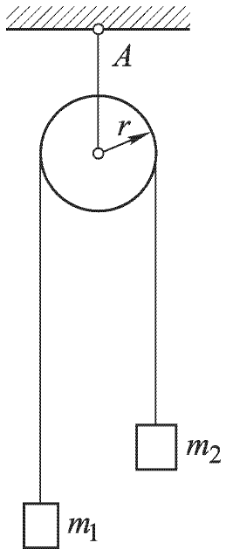
\includegraphics[width=0.6\textwidth]{AtwoodInertia.png}
\caption{}
\label{AtwoodInertia}
\end{subfigure}%
\begin{subfigure}{.33\textwidth}
  \centering
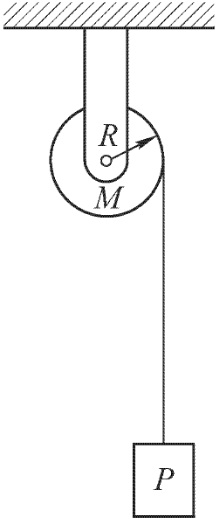
\includegraphics[width=0.6\textwidth]{CylinderInertia.png}
\caption{}
\label{CylinderInertia}
\end{subfigure}
\begin{subfigure}{.33\textwidth}
  \centering
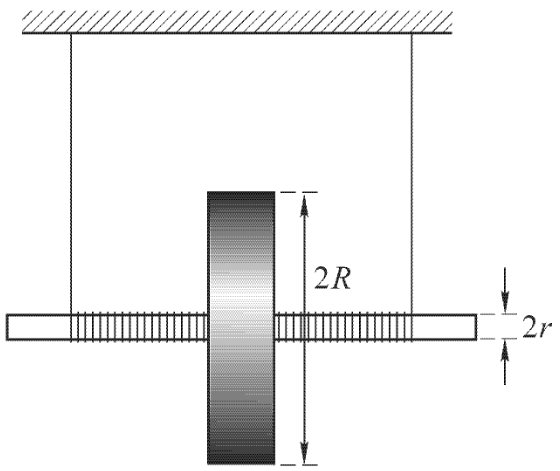
\includegraphics[width=1.2\textwidth]{MaxwellDisk.png}
\caption{}
\label{MaxwellDisk}
\end{subfigure}
\caption{}
\end{figure}
%Сив319
\AddProb Схема демонстрационного прибора (диск Максвелла) изображена на рис. \ref{MaxwellDisk}. На валик радиусом $r$ наглухо насажен сплошной диск радиуса $R$ и массы $M$. Валик и диск сделаны из одного материала, причем выступающие из диска части оси имеют массу $m$. К валику прикреплены нити одинаковой длины, при помощи которых прибор подвешивается к штативу. На валик симметрично наматываются нити в один ряд, благодаря чему диск поднимается, а затем предоставляют диску свободно опускаться. Найти ускорение, с которым опускается диск.
%Сив325
\AddProb По наклонной плоскости, образующей угол $\alpha$ с горизонтом, скатывается без скольжения сплошной однородный диск. Найти линейное ускорение $a$ центра диска.

%Сив333
\begin{wrapfigure}[9]{r}{6cm}
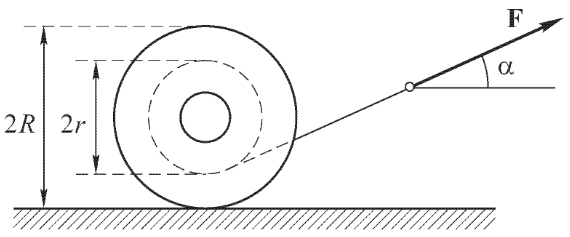
\includegraphics[width=0.5\textwidth]{Coil.png}
\caption{}
\label{Coil}
\end{wrapfigure}
\AddProb На горизонтальной плоскости лежит катушка ниток. С каким
ускорением $a$ будет двигаться ось катушки, если тянуть за нитку с силой $F$ (рис. \ref{Coil})? Каким образом	надо тянуть за нитку, чтобы катушка двигалась в сторону натянутой нитки? Катушка движется по поверхности стола без скольжения. Найти силу трения между катушкой и столом.

%Сив316
\begin{wrapfigure}[13]{r}{2.5cm}
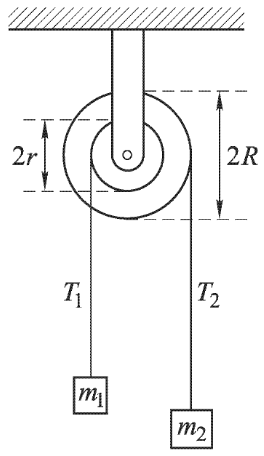
\includegraphics[width=0.25\textwidth]{2BlocksInertia.png}
\caption{}
\label{2BlocksInertia}
\end{wrapfigure}
\AddProb На ступенчатый цилиндрический блок намотаны в противоположных направлениях две легкие нити, нагруженные массами $m_1$ и $m_2$ (рис. \ref{2BlocksInertia}). Найти угловое ускорение блока и натяжения $T_1$ и $T_2$ нитей, учитывая момент инерции $I$ блока.
%Сив317
\AddProb Модель ворота укреплена на одной чашке весов (рис. \ref{weighter}). На ворот с моментом инерции $I$ намотана нить с грузиком массы $m$. Весы уравновешены, когда ворот заторможен, и нить не разматывается. Насколько следует изменить вес гирь на другой чашке весов для того, чтобы восстановить равновесие, когда ворот вращается под действием опускающегося вниз грузика?

\begin{figure}[h]
\centering
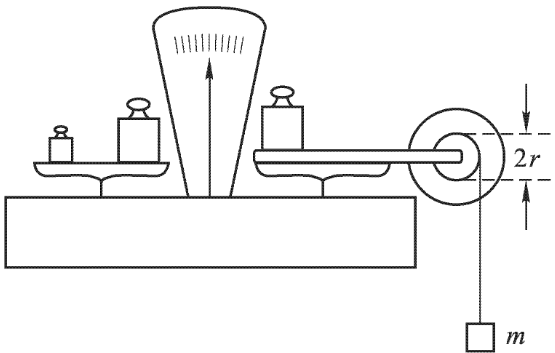
\includegraphics[width=0.4\textwidth]{weighter.png}
\caption{}
\label{weighter}
\end{figure}
%Сив323
\begin{wrapfigure}[9]{r}{3cm}
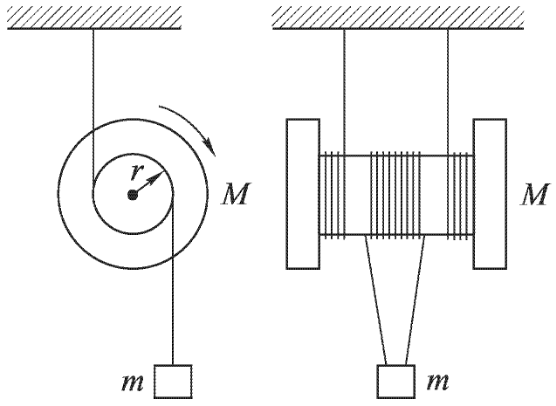
\includegraphics[width=0.3\textwidth]{coil2Threads.png}
\caption{}
\label{coil2Threads}
\end{wrapfigure}
\AddProb С каким ускорением $a$ будет опускаться катушка с массой $M$ и моментом инерции $i$ относительно оси симметрии, если она подвешена аналогично диску Максвелла (рис. \ref{coil2Threads}). На катушку намотаны еще две нити, к которым подвешен груз массы $m$. Определить натяжения нитей.
%Сив326
\AddProb Найти ускорение $a$ центра однородного шара, скатывающегося без скольжения по наклонной плоскости, образующей угол $\alpha$ с горизонтом. Чему равна сила трения сцепления шара и плоскости?
%Сив328
\AddProb По наклонной плоскости, составляющей с горизонтом угол $\alpha = 30^{\circ}$, скатывается без скольжения сплошной однородный цилиндр, масса которого равна 300 г. Найти величину силы трения цилиндра о плоскость.
%Сив329
\AddProb Какова должна быть величина коэффициента трения $\mu$, чтобы однородный цилиндр скатывался без скольжения с наклонной 
плоскости, образующей угол $\alpha$ с горизонтом?
%Сив332
\AddProb К тележке, стоящей на горизонтальной плоскости, привязана
нить, перекинутая через блок, укрепленный у края стола; к концу нити прикреплен груз массы $m_3$ = 500 г. Определить ускорение тележки $a$, если известно, что масса платформы тележки $m_1$ = 1,4 кг, масса каждого колеса $m_2$ = 400 г и колеса представляют собой сплошные диски. Колеса катятся по поверхности стола без скольжения, а трение качения отсутствует.
\clearpage